\documentclass[border=1pt]{standalone}
%\usepackage[dvipsnames]{xcolor}
\usepackage{tikz}                       % Graphen und kommutative Diagramme
\usetikzlibrary{patterns}               % Um schraffierte Formen in der tikzpicture-Umgebung zu zeichnen.
\usetikzlibrary{shapes}                 % Polygone
\newcommand{\ul}[1]{\underline{\smash{#1}}}

\begin{document}
\centering
\resizebox{!}{2.3cm}{
    \raisebox{-0.5\height}{
        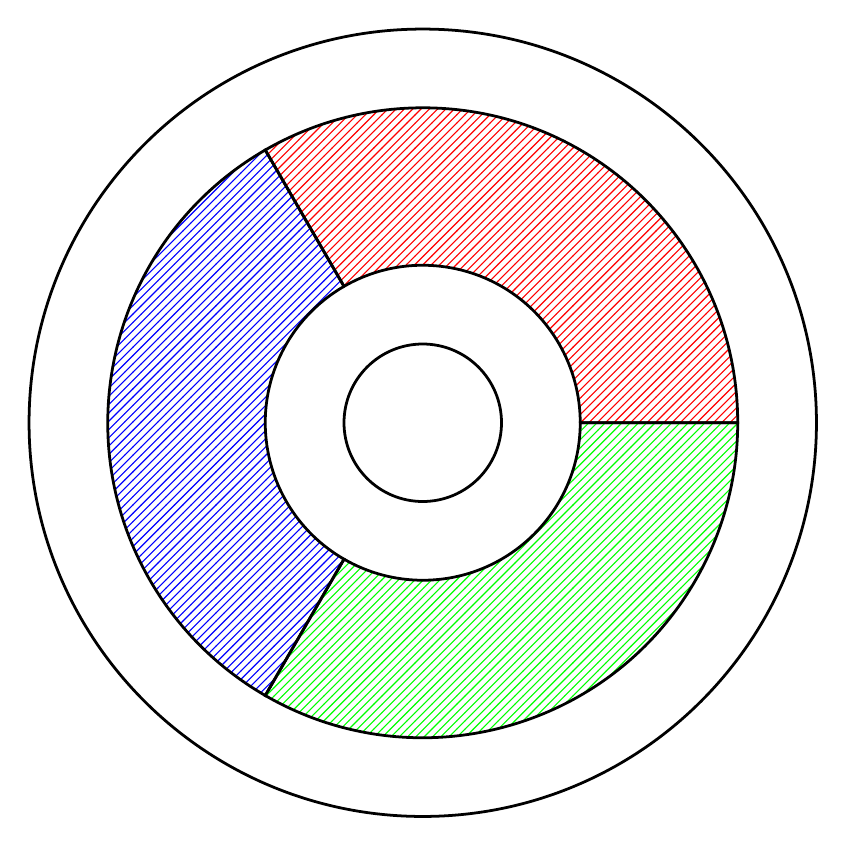
\begin{tikzpicture}[line width=1pt]
            % draw shaded slit box
            \filldraw[pattern=north east lines, pattern color=red] 
            (0 : 2) -- (  0 : 4) arc [radius = 4, start angle =   0, delta angle =  120] 
                    -- (120 : 2) arc [radius = 2, start angle = 120, delta angle = -120] ;
            
            \filldraw[pattern=north east lines, pattern color=blue] 
            (120 : 2) -- (120 : 4) arc [radius = 4, start angle = 120, delta angle =  120] 
                      -- (240 : 2) arc [radius = 2, start angle = 240, delta angle = -120] ;
            
            \filldraw[pattern=north east lines, pattern color=green] 
            (240 : 2) -- (240 : 4) arc [radius = 4, start angle = 240, delta angle =  120] 
                      -- (360 : 2) arc [radius = 2, start angle =   0, delta angle = -120] ;
                    
            % draw inner and outer circles
            \draw[color=black] (0, 0) circle (1);
            \draw[color=black] (0, 0) circle (5);
        \end{tikzpicture}
    }
    \hspace{4cm}
    \raisebox{-0.5\height}{
        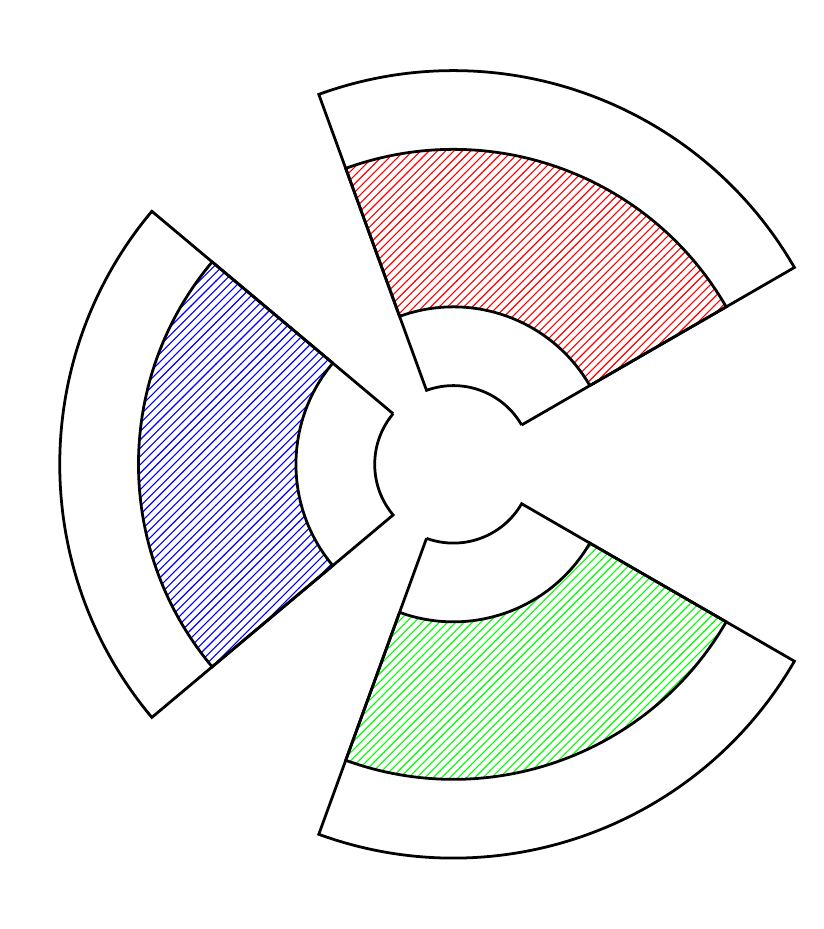
\begin{tikzpicture}[line width=1pt]
            % draw shaded slit box
            \filldraw[pattern=north east lines, pattern color=red] 
            ( 30 : 2) -- ( 30 : 4) arc [radius = 4, start angle =  30, delta angle =  80] 
                      -- (110 : 2) arc [radius = 2, start angle = 110, delta angle = -80] ;
            \filldraw[pattern=north east lines, pattern color=blue] 
            (140 : 2) -- (140 : 4) arc [radius = 4, start angle = 140, delta angle =  80] 
                      -- (220 : 2) arc [radius = 2, start angle = 220, delta angle = -80] ;
            \filldraw[pattern=north east lines, pattern color=green] 
            (250 : 2) -- (250 : 4) arc [radius = 4, start angle = 250, delta angle =  80] 
                      -- (330 : 2) arc [radius = 2, start angle = 330, delta angle = -80] ;
                    
            % draw pieces of cake
            \draw ( 30 : 1) -- ( 30 : 5) arc [radius = 5, start angle =  30, delta angle =  80] 
                            -- (110 : 1) arc [radius = 1, start angle = 110, delta angle = -80];
            \draw (140 : 1) -- (140 : 5) arc [radius = 5, start angle = 140, delta angle =  80] 
                            -- (220 : 1) arc [radius = 1, start angle = 220, delta angle = -80];
            \draw (250 : 1) -- (250 : 5) arc [radius = 5, start angle = 250, delta angle =  80] 
                            -- (330 : 1) arc [radius = 1, start angle = 330, delta angle = -80];
        \end{tikzpicture}
    }
    \hspace{4cm}
    \raisebox{-0.5\height}{
        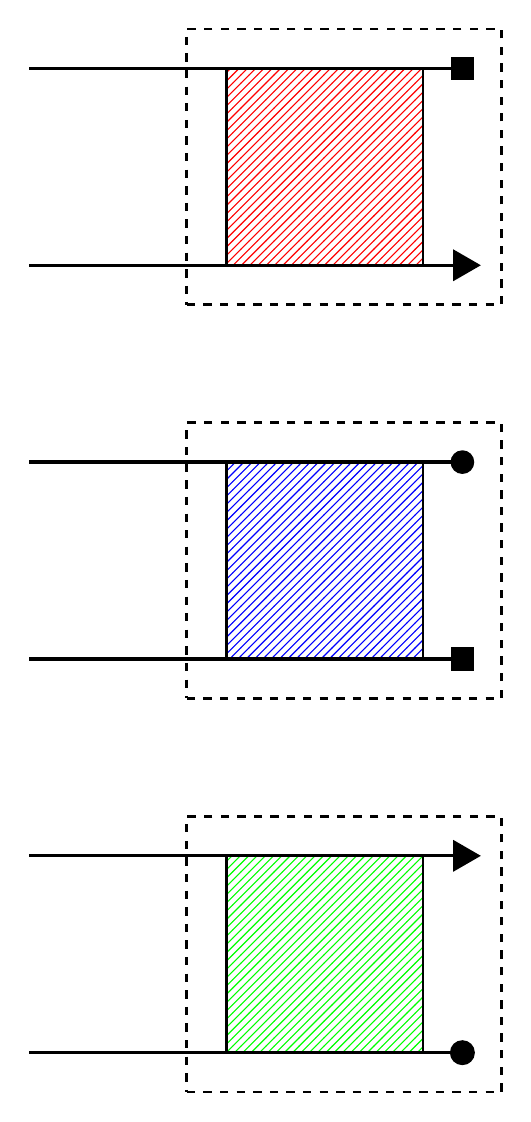
\begin{tikzpicture}[line width=1pt]
            %%%%%%%%
            % red picture
            %%%%%%%%
            
            % draw shaded slit box
            \filldraw[pattern=north east lines, pattern color=red] (.5, 10.5) -- (3, 10.5) -- (3, 13) -- (.5, 13) -- (.5, 10.5);
            
            % draw line
            \draw[dashed] (0, 10) -- (4, 10) -- (4, 13.5) -- (0, 13.5) -- (0, 13) -- (0,10);
            
            % draw slits
            \draw[color=black, line width=1.2pt] (-2, 10.5) -- (3.5, 10.5);
            \draw[color=black, line width=1.2pt] (-2, 13) -- (3.5, 13);
            \node[rotate = 270, scale = 0.6, draw = black, fill = black, regular polygon, regular polygon sides = 3] at (3.5, 10.5) {};
            \node[scale = 0.8, draw = black, fill = black, regular polygon, regular polygon sides = 4] at (3.5, 13) {};
            
            %%%%%%%%
            % blue picture
            %%%%%%%%
            
            % draw shaded slit box
            \filldraw[pattern=north east lines, pattern color=blue] (.5, 5.5) -- (3, 5.5) -- (3, 8) -- (.5, 8) -- (.5, 5.5);
            
            %draw line
            \draw[line width=1pt, dashed] (0, 5) -- (4, 5) -- (4, 8.5) -- (0, 8.5) -- (0, 8) -- (0,5);
            
            % draw slits
            \draw[color=black, line width=1.2pt] (-2, 5.5) -- (3.5, 5.5);
            \draw[color=black, line width=1.2pt] (-2, 8) -- (3.5, 8);
            \node[scale = 0.8, draw = black, fill = black, regular polygon, regular polygon sides = 4] at (3.5, 5.5) {};
            \node[scale = 0.8, draw = black, fill = black, circle] at (3.5, 8) {};
            %%%%%%%%
            % green picture
            %%%%%%%%
            
            % draw shaded slit box
            \filldraw[pattern=north east lines, pattern color=green] (.5, 0.5) -- (3, 0.5) -- (3, 3) -- (.5, 3) -- (.5, 0.5);
            
            % draw line
            \draw[dashed] (0, 0) -- (4, 0) -- (4, 3.5) -- (0, 3.5) -- (0, 3) -- (0,0);
            
            % draw slits
            \draw[color=black, line width=1.2pt] (-2, 0.5) -- (3.5, 0.5);
            \draw[color=black, line width=1.2pt] (-2, 3) -- (3.5, 3);
            \filldraw (3.5, 0.5) circle (4pt);
            \node[rotate = 270, scale = 0.6, draw = black, fill = black, regular polygon, regular polygon sides = 3] at (3.5, 3) {};
        \end{tikzpicture}
    }
}
\end{document}
